\section{Experimental settings}
\label{app:configuration}
Table~\ref{tab:config} specifies the model, experience, and execution settings used in evaluation. We use the official GroundSG checkpoint trained on the RoboMME training split, and training demonstrations also provide the initial duration advice. During testing, experience updates follow the schedule in Section~\ref{sec:setup}. Global advice is shared across tasks, while all 37 accepted updates during the formal evaluation are task-specific. Each episode uses a fixed version of the experience store.

\begin{table}[ht]
\caption{Evaluation settings. Control limits apply to actual executed control steps, including interventions.}
\label{tab:config}
\small
\begin{tabularx}{\linewidth}{@{}p{0.32\linewidth}X@{}}
\toprule
Setting & Value \\
\midrule
Astra model and reasoning setting & GPT-6 Astra; high reasoning effort \\
VLA checkpoint and inference & Official RoboMME GroundSG (\pifive), training step 79,999; inference seed 42 with independent random state per connection \\
Environment control frequency & 20 Hz \\
Camera observations & Front and wrist RGB images \\
Sparse history query & Up to eight uniformly sampled frames, including endpoints \\
Delegation budget range & 30 to 200, in increments of 10 control steps \\
Executed actions per VLA prediction & Up to the first 16 predicted actions, limited by the remaining execution budget \\
Episode API limit & 80 calls; 8,192 output tokens per call; 300,000-token context limit \\
Cross-task experience & Shared global advice and separate task experience; fixed version per episode \\
Paired comparison sample & Ten StopCube seeds; 1,000 control steps per run; no experience updates \\
Compute and serving & Paired experiment: one NVIDIA A100 80GB for the VLA, dual Intel Xeon Platinum 8358P CPUs for simulation; Astra via remote API \\
\bottomrule
\end{tabularx}
\end{table}

\paragraph{Robot-state monitors.}
The measured gripper monitor detects a total finger-width change of at least 5\,mm from the start of the execution interval, sustained for two measured samples in the same direction. The direction monitor checks predicted or measured displacement greater than 20\,mm in a selected signed world-frame direction relative to the robot pose at the start of the execution interval. The stationary-motion monitor uses a position diameter of at most 2\,mm and an orientation diameter of at most $2^\circ$ over 32 control steps. An impending gripper-command switch can also trigger review. Astra selects the active monitors for each execution interval. Budget exhaustion prompts review, and episode termination stops execution.

\section{Per-task performance and execution allocation}
\label{app:task-results}
Table~\ref{tab:task-results} reports success and execution allocation for each task. Automatic continuation counts execution after the first chunk of an execution interval. The control fraction includes direct Astra interventions in its denominator. Each task contributes 50 episodes, and pooled allocation fractions weight tasks by their executed chunk or control counts.

\begin{table}[ht]
\centering
\caption{Per-task results. SR: success rate; auto chunks: automatic continuation as a fraction of all VLA chunks; auto control steps: automatic continuation as a fraction of all executed control steps. All entries are percentages.}
\label{tab:task-results}
\small
\begin{tabular}{@{}llrrr@{}}
\toprule
Category & Task & SR (\%) & Auto chunks (\%) & Auto control steps (\%) \\
\midrule
Counting & BinFill & 96.0 & 63.61 & 60.41 \\
 & StopCube & 96.0 & 65.15 & 68.87 \\
 & PickXtimes & 100.0 & 53.95 & 49.13 \\
 & SwingXtimes & 96.0 & 46.87 & 45.20 \\
\midrule
Permanence & ButtonUnmask & 100.0 & 73.84 & 69.51 \\
 & VideoUnmask & 100.0 & 73.88 & 71.42 \\
 & VideoUnmaskSwap & 98.0 & 69.11 & 65.87 \\
 & ButtonUnmaskSwap & 92.0 & 50.26 & 41.35 \\
\midrule
Reference & PickHighlight & 100.0 & 71.43 & 69.17 \\
 & VideoRepick & 100.0 & 67.55 & 63.03 \\
 & VideoPlaceButton & 98.0 & 76.26 & 75.36 \\
 & VideoPlaceOrder & 90.0 & 63.44 & 65.93 \\
\midrule
Imitation & MoveCube & 100.0 & 53.30 & 48.64 \\
 & InsertPeg & 90.0 & 29.06 & 29.01 \\
 & PatternLock & 100.0 & 35.62 & 34.06 \\
 & RouteStick & 98.0 & 25.65 & 22.30 \\
\midrule
\multicolumn{2}{@{}l}{Overall / pooled} & 97.1 & 58.11 & 54.93 \\
\bottomrule
\end{tabular}
\end{table}

\section{Interface and experience details}
\label{app:interfaces}
\paragraph{Observation provenance.}
Image-delivery records distinguish the visual evidence included in each successful Astra request from observations available only through retrospective inspection of the full recording.

\paragraph{Grounding.}
For a front image of height $H$ and width $W$, a normalized point $(y_n,x_n)\in[0,1000]^2$ is converted to
\begin{equation}
 y=\min(\lfloor y_nH/1000\rfloor,H-1),\qquad
 x=\min(\lfloor x_nW/1000\rfloor,W-1).
\end{equation}
The pixel coordinates replace the instruction's ordered point slots. Validation checks finite coordinate values, normalized bounds, the number of supplied points, and compatibility with the task's templates and permitted attributes. Astra can inspect an overlay before setting the subgoal. The default sparse history query selects up to eight uniformly spaced frames, including interval endpoints.

\paragraph{Control steps and duration priors.}
A control step is counted at the shared environment action interface, separately from simulator integration steps. At environment frequency $f_c=20\,\mathrm{Hz}$, $n$ steps correspond nominally to $n/f_c$ seconds of simulated control. Inference and API waiting time contribute separately to elapsed time. Repeated training samples are deduplicated by task, episode, and timestep before consecutive identical subgoal labels are grouped. Segment lengths are estimated from timestep differences. For lengths $D_s$ associated with subgoal $s$, the initial recommendation is
\begin{equation}
 \widehat B_s=\min\!\left(200,10\left\lfloor Q_{0.25}(D_s)/10\right\rfloor\right).
\end{equation}
Recommendations below 30 control steps become advice for close review. Because sampled annotations may miss short segments or include trailing frames in terminal segments, these duration estimates serve as initial guidance rather than exact subtask boundaries.

\paragraph{Experience validation and applicability.}
Submission checks cover required fields, permitted scope and applicability labels, cited frame indices, and the existence of superseded identifiers. Scheduling advice is also checked for compatibility with subgoal templates and valid monitor parameters. Experience entries are marked as either policy-independent or specific to a review policy. When retrieving advice, the harness first selects entries applicable to the current policy and then resolves superseded recommendations. The optional scheduling field \texttt{max\_trust\_steps} records a recommended review interval; the configured execution maximum remains the enforced limit.

\section{Measurement definitions}
\label{app:measurements}
Success rate is the number of officially successful episodes divided by the evaluated count. Equal task sizes make overall success equal to the mean task success rate. Execution-time summaries include only the 777 successful episodes; token totals include all 800 episodes. API attempts and elapsed time include failed requests. Token statistics report coverage of returned usage; cached input is a subset of total input, and missing usage remains unknown. Execution and post-episode revision token totals are reported separately. API latency for revision is not a measurement of the complete revision wall time.

Automatic continuation counts VLA chunks executed after the first chunk of an execution interval. The all-chunk fraction divides these by all executed VLA chunks. The automatic-control fraction divides control steps in continuation chunks by all executed control steps, including direct interventions. Fractions use pooled counts across episodes rather than averages of episode percentages.

\begin{table}[!htbp]
\centering
\caption{Execution allocation across all 800 episodes. Each row counts executed robot-control requests (VLA chunks or direct intervention segments); direct interventions can have different lengths from VLA chunks. Percentages use pooled counts.}
\label{tab:allocation-detail}
\small
\begin{tabularx}{\linewidth}{@{}Xrrrr@{}}
\toprule
Execution mode & Requests & Share (\%) & Control steps & Share (\%) \\
\midrule
Subgoal entry & 2,829 & 15.88 & 44,709 & 17.23 \\
Astra intervention & 587 & 3.29 & 12,752 & 4.91 \\
Automatic VLA continuation & 10,014 & 56.20 & 142,516 & 54.93 \\
VLA continuation after review & 4,390 & 24.64 & 59,495 & 22.93 \\
\midrule
Total & 17,820 & 100.00 & 259,472 & 100.00 \\
\bottomrule
\end{tabularx}
\end{table}

\FloatBarrier
\section{Successful-episode execution time}
\label{app:completion-time}
Execution time runs from environment readiness to the end of robot execution, excluding startup and post-episode review. The pooled row summarizes all 777 successful episodes, rather than averaging task means. P90 uses linear interpolation between ordered observations.
\paragraph{Interpretation of completion times.}
Across 777 successful episodes, mean completion time is 513.7 seconds, the median is 390.5 seconds, and the 90th percentile is 1,102.0 seconds. Task means range from 141.2 seconds on VideoUnmask to 991.8 seconds on ButtonUnmaskSwap. These measurements include model inference, history queries, action execution, and waiting; API load and network conditions also affect them. These full-benchmark timing results are descriptive and are not intended as controlled efficiency comparisons with published systems. The matched StopCube experiment provides a controlled comparison of review policies.

\begin{table}[!htbp]
\centering\small
\caption{Completion times for successful episodes. All times are seconds.}
\begin{tabular}{@{}lrrrr@{}}
\toprule
Task & Successful episodes & Mean & Median & P90 \\
\midrule
BinFill & 48 & 802.1 & 800.1 & 1378.9 \\
StopCube & 48 & 416.6 & 385.1 & 615.0 \\
PickXtimes & 50 & 712.2 & 602.6 & 1315.3 \\
SwingXtimes & 48 & 887.3 & 913.3 & 1340.5 \\
ButtonUnmask & 50 & 359.0 & 267.4 & 726.2 \\
VideoUnmask & 50 & 141.2 & 111.5 & 237.1 \\
VideoUnmaskSwap & 49 & 383.5 & 288.8 & 690.5 \\
ButtonUnmaskSwap & 46 & 991.8 & 916.6 & 1319.7 \\
PickHighlight & 50 & 385.1 & 352.6 & 610.3 \\
VideoRepick & 50 & 782.9 & 645.0 & 1239.5 \\
VideoPlaceButton & 49 & 306.7 & 281.4 & 413.3 \\
VideoPlaceOrder & 45 & 254.1 & 244.3 & 341.0 \\
MoveCube & 50 & 296.2 & 160.8 & 690.7 \\
InsertPeg & 45 & 760.1 & 719.6 & 1150.8 \\
PatternLock & 50 & 249.5 & 224.4 & 461.0 \\
RouteStick & 49 & 544.1 & 494.0 & 880.1 \\
\midrule
Overall / pooled & 777 & 513.7 & 390.5 & 1,102.0 \\
\bottomrule
\end{tabular}
\end{table}

\FloatBarrier
\section{Monitor selection and resource use}
Monitor selection is counted once per execution interval, across 3,541 intervals. Several monitors may be selected together, so selection shares need not sum to 100\%. No optional monitor is selected in 1,840 intervals (51.96\%); budgets and mandatory termination conditions still apply. Trigger frequency counts intervals ending with a detected condition and does not measure error-detection accuracy.
\begin{table}[!htbp]
\centering\small
\caption{Monitor selection and subsequent triggering. The 28 direction triggers all concern proposed motion; none comes from measured directional displacement.}
\begin{tabularx}{\linewidth}{@{}Xrrr@{}}
\toprule
Monitor & Selected & Share (\%) & Triggered / selected (\%) \\
\midrule
Before gripper-command switch & 1,062 & 29.99 & 28.91 \\
Measured gripper-width change & 354 & 10.00 & 70.34 \\
Selected-direction displacement & 244 & 6.89 & 11.48 \\
Stationary motion & 120 & 3.39 & 0.00 \\
\bottomrule
\end{tabularx}
\end{table}

Selection differs by task stage. On StopCube, all 51 button-preparation intervals omit optional monitors, whereas 56 of 85 stationary-waiting intervals select a direction monitor. On SwingXtimes, a pre-command gripper monitor is selected in 186 of 193 target-movement intervals (96.37\%), compared with 22 of 93 grasping intervals (23.66\%). On PickXtimes, the stationary-motion monitor is selected in 49 of 50 button-stop intervals, yet it never triggers across the evaluation.

\begin{table}[!htbp]
\centering\small
\caption{Mean recorded token usage per evaluated episode, over all 800 episodes. Cached input is a subset of input.}
\begin{tabular}{@{}lrr@{}}
\toprule
Tokens & Execution & Post-episode review \\
\midrule
Input & 1,790,701.2 & 318,456.8 \\
Cached input & 1,633,224.3 & 308,963.6 \\
Uncached input & 157,476.9 & 9,493.2 \\
Output & 2,724.9 & 674.2 \\
\bottomrule
\end{tabular}
\end{table}
All 19,061 successful API responses include usage records, while 112 failed attempts have unknown usage, giving 99.4\% coverage. Reported per-episode means use recorded usage divided by all 800 episodes and may underestimate actual token consumption. They should not be interpreted as billing estimates.

\FloatBarrier
\section{Within-episode case sequences}
\label{app:case-sequences}
Figure~\ref{fig:within-episode-cases} expands the cross-episode examples in Figures~\ref{fig:trace} and~\ref{fig:history-case} with two frames from the same episode in each pair.

\begin{casefigure}
\begin{minipage}[t]{0.48\linewidth}
\centering
{\small\bfseries (a) PickXtimes / episode 2\par}
\vspace{4pt}
\begin{minipage}[t]{0.43\linewidth}\centering
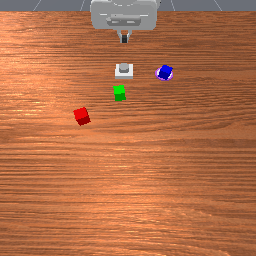
\includegraphics[width=\linewidth]{supplementary/20261023-stopcube/figures/PickXtimes-ep2-f288-front.png}\par
{\scriptsize Frame 288\par Budget exhausted; review\par}
\end{minipage}\hfill
\begin{minipage}[t]{0.43\linewidth}\centering
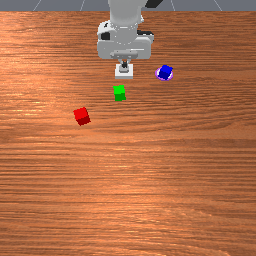
\includegraphics[width=\linewidth]{supplementary/20261023-stopcube/figures/PickXtimes-ep2-f301-front.png}\par
{\scriptsize Frame 301\par Official success\par}
\end{minipage}\par\vspace{4pt}
{\footnotesize $16+16+16+12=60$ steps $\rightarrow$ review\par
Another 13 control steps $\rightarrow$ success\par}
\end{minipage}\hfill
\begin{minipage}[t]{0.48\linewidth}
\centering
{\small\bfseries (b) VideoPlaceButton / episode 3\par}
\vspace{4pt}
\begin{minipage}[t]{0.43\linewidth}\centering
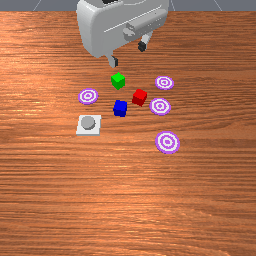
\includegraphics[width=\linewidth]{supplementary/20261023-stopcube/figures/VideoPlaceButton-ep3-f679-front.png}\par
{\scriptsize Frame 679\par Before the late swap\par}
\end{minipage}\hfill
\begin{minipage}[t]{0.43\linewidth}\centering
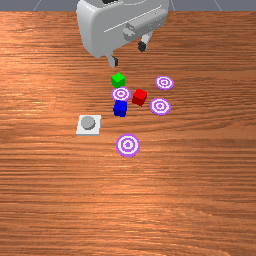
\includegraphics[width=\linewidth]{supplementary/20261023-stopcube/figures/VideoPlaceButton-ep3-f700-front.png}\par
{\scriptsize Frame 700\par After the late swap\par}
\end{minipage}\par\vspace{4pt}
{\footnotesize Late changes in ring positions\par
Both frames inspected after failure\par}
\end{minipage}
\caption{Two within-episode sequences, read left to right within each pair. (a) Astra reviews execution after the revised 60-step budget and permits another chunk; official feedback reports success after 13 further steps. (b) Historical frames show the late ring permutation examined during post-episode review. The pairs document execution and historical evidence, respectively.}
\label{fig:within-episode-cases}
\end{casefigure}

\FloatBarrier
\section{Failure annotation and reference-frame clarification}
\label{app:failure-analysis}
Manual inspection of the 23 unsuccessful episodes assigns one primary label per episode: historical interpretation (8), subgoal grounding (1), execution (9), or review and recovery (5). The execution category includes two SwingXtimes episodes in which the motion does not fully reach the target and one VideoUnmaskSwap episode with insufficient container lift. Each episode is counted once according to its primary failure mode.

In the first RouteStick episode, Astra misinterprets the task's left--right convention, leading to an incorrect directional subgoal. As RoboMME's directional instructions do not explicitly specify the reference frame, we subsequently added a clarification of this convention to the agent's global experience context: task directions refer to the initial wrist view or initial robot orientation, rather than the changing wrist orientation or the front-view screen axes. Image points retain the pixel coordinates of their own camera. This interface clarification is not counted among the 37 autonomous experience updates.

\begin{casefigure}
{\small\bfseries (a) VideoPlaceOrder / episode 11\par}\vspace{3pt}
\caseframe{VideoPlaceOrder-ep11-f491}{Frame 491: remembered location}{Target initially at the lower right}\hfill
\caseframe{VideoPlaceOrder-ep11-f740}{Frame 740: late permutation}{Inspected retrospectively}\hfill
\caseframe{VideoPlaceOrder-ep11-f1012}{Frame 1012: incorrect selection}{Old screen location reused}\par\vspace{8pt}
{\small\bfseries (b) ButtonUnmaskSwap / episode 17\par}\vspace{3pt}
\caseframe{ButtonUnmaskSwap-ep17-f98}{Frame 98: brief button contact}{First button press}\hfill
\caseframe{ButtonUnmaskSwap-ep17-f218}{Frame 218: premature transition}{Container manipulation begins}\hfill
\caseframe{ButtonUnmaskSwap-ep17-f612}{Frame 612: delayed recovery}{Button action revisited}\par\vspace{8pt}
{\small\bfseries (c) InsertPeg / episode 0\par}\vspace{3pt}
\caseframe{InsertPeg-ep0-f441}{Frame 441: incorrect transport}{Direction monitor triggers review}\hfill
\caseframe{InsertPeg-ep0-f633}{Frame 633: alignment attempts}{Contact recovery remains unsuccessful}\hfill
\caseframe{InsertPeg-ep0-f723}{Frame 723: incomplete insertion}{Episode ends without completion}
\caption{Representative failures, read left to right within each episode. (a) VideoPlaceOrder loses target identity through a late ring swap; frame 740 was inspected retrospectively. (b) ButtonUnmaskSwap moves to container manipulation too early and later retries the button. (c) InsertPeg remains incomplete after repeated alignment and contact recovery.}
\label{fig:failures}
\end{casefigure}

\FloatBarrier


\section{Review-policy comparison}
\label{app:paired}
The StopCube comparison uses ten official test seeds, with both policies rerun under the same harness configuration. The two conditions receive identical saved versions of the experience store within each pair. Experience updates are disabled to keep the comparison focused on review policy. Runs alternate which policy executes first.

Delegation is faster on all nine jointly successful seeds, saving a mean of 227.6 seconds. The first per-chunk run includes 35.5 seconds of VLA inference, compared with 2.3 seconds for its delegated counterpart. Excluding this pair leaves eight joint successes with mean times of 491.9 and 280.6 seconds, respectively, a 43.0\% reduction. Across all ten runs, execution uses 2,021 control steps with per-chunk review and 2,010 with delegation. Input-token totals fall from 30.63 to 12.05 million; uncached input falls from 2.22 to 1.19 million, and output from 32,222 to 21,333 tokens.
